%%%%%%%%%%%%%%%%%%%%%%%%%%%%%%%%%%%%%%%%%%%%%%%%%%%%%%%%%%%%%%%%%%%%%%
% How to use writeLaTeX: 
%
% You edit the source code here on the left, and the preview on the
% right shows you the result within a few seconds.
%
% Bookmark this page and share the URL with your co-authors. They can
% edit at the same time!
%
% You can upload figures, bibliographies, custom classes and
% styles using the files menu.
%
%%%%%%%%%%%%%%%%%%%%%%%%%%%%%%%%%%%%%%%%%%%%%%%%%%%%%%%%%%%%%%%%%%%%%%

\documentclass[12pt]{article}

\usepackage{sbc-template}

\usepackage{graphicx,url}

\usepackage[brazil]{babel}   
\usepackage[utf8]{inputenc}  

%Inclui () nas citações
\usepackage{cite}
\renewcommand\citeleft{(}
\renewcommand\citeright{)}



     
\sloppy

\title{Classificação de células tumorais em imagens\\ histopatológicas utilizando Deep Learning}

\author{Breno C. Zukowski\inst{1}, Lucas B. Figueira\inst{1}}


\address{Faculdade de Tecnologia de Ribeirão Preto - (FATEC)\\
  Ribeirão Preto, SP -- Brasil
  \email{breno.marques@fatec.sp.gov.br, lucas.figueira@fatec.sp.gov.br}
}

\begin{document}

\maketitle

\begin{abstract}
  Diagnosing breast cancer can be challenging and laborious even for well-trained professionals.
  Inexperienced physicians and disagreement among histopathologists are primary causes of misdiagnosis
  that compromise patient care. With computational decision support systems using deep learning,
  it is possible to guarantee better results for this process. This article demonstrates the use
  of a Convolutional Neural Network model for this purpose.
\end{abstract}

\begin{resumo}
  O diagnóstico de câncer de mama pode ser desafiador e laborioso mesmo para profissionais bem treinados.
  Médicos inexperientes e discordância entre histopatologistas são causadores primários de diagnósticos errôneos
  que comprometem o tratamento de pacientes. Com sistemas computacionais de apoio a decisão utilizando deep learning,
  é possível garantir melhores resultados para este processo. Este artigo demonstra a utilização
  de um modelo Rede Neural Convolucional para tal finalidade.
\end{resumo}


\section{Introdução}

O câncer de mama é a mais recorrente neoplasia maligna em mulheres ao redor do mundo. Apenas em 2020 foram realizados 2,3 milhões de diagnósticos e 685.000 mortes foram registradas \cite{who2021}. No Brasil, o cenário é similar: no mesmo ano a ordem de incidência estava prevista para cerca de 600.000 casos \cite{inca2018}. A análise de imagens histológicas está entre os mais utilizados métodos de diagnóstico da atualidade. Porém, existem deficiências associadas ao método provenientes do trabalho humano desenvolvido para realizá-lo. Falhas estas, que podem levar a diagnósticos errados e agravamento do quadro de saúde do paciente em decorrência da falta de tratamento imediato. Mesmo quando bem sucedidos, a análise humana demanda uma grande carga de esforço e tempo que poderiam ser mitigados com auxílio de visão computacional e deep learning.

Segundo \cite{tiezzi2020}, uma série de fatores podem ser descritos como métodos de predição de prognóstico, sendo atualmente utilizados no contexto clínico para determinação de tratamento, em especial para utilização de drogas antineoplásicas. Dentre eles destacam-se critérios clínicos, histológicos e utilização de marcadores tumorais. Abordando o critério histológico, temos o grau de diferenciação tumoral, baseado no sistema de escore de Nottingham (NGS), que, apesar de ser considerado um potente método de predição, recebe críticas em relação à sua baixa reprodutibilidade, provavelmente devido ao seu caráter subjetivo e processamento pré-analítico da amostra. Dessa forma, gera ampla discordância entre histologistas que o aplicam, o que impacta diretamente no prognóstico do paciente e na decisão clínica de administrar ou não a quimioterapia sistêmica.
Alternativas de métodos com biologia molecular vêm sendo propostas para inferir com maior acurácia o estágio de agressividade da doença de forma a evitar desvios de diagnóstico. Entretanto, essas são técnicas de alto custo, inviáveis em muitas situações, principalmente em países subdesenvolvidos.

Atualmente, as técnicas de aprendizado de máquina vêm ganhando espaço em diversas áreas e aplicações. Na medicina, já são importantes métodos de auxílio ao diagnóstico de imagens radiológicas \cite{hu2018}. Diversos modelos computacionais têm sido desenvolvidos nos últimos anos utilizando a metodologia deep learning para concretizar sistemas de apoio ao diagnóstico. Grupos de pesquisa ao redor do mundo têm desenvolvido soluções de aprendizado de máquina utilizando técnicas diversas de deep learning, que, apesar de rápidas e geralmente acuradas, apenas oferecem mapas de calor e pontos de atenção, informações insuficientes para interpretação concreta e justificação do diagnóstico oferecido pela máquina, o que não é adequado para sistemas de apoio à decisão médica \cite{li2021}.

Vê-se, portanto, nas R-CNNs (do inglês, Region-Based Convolutional Neural Network) uma solução viável para análise de recortes específicos de tecido com a quantidade de informação e assertividade adequadas para auxílio ao diagnóstico médico. Pois a partir delas é possível segmentar e classificar regiões de interesse com as informações necessárias para evidenciar a presença de tumores malignos com eficiência.


\section{Revisão bibliográfica}

\subsection*{Introdução}
Ao discutir-se R-CNN's é primeiro importante entender os conceitos que embasam as CNN's (do inglês, {\it Convolutional Neural Networks}), algoritmos de aprendizagem profunda especializados em processamento e classificação de imagens. Segundo \cite{Goodfellow-et-al-2016} redes neurais convolucionais são um tipo especializado de rede neural para processamento de dados organizados topologicamente em grades, que através de operações matemáticas chamadas convoluções, são capazes de extrair características principais das entradas utilizando filtros (kernels), garantindo eficiência e redução de custos computacionais para a classificação.

Diferentemente de outros tipos de dados, imagens possuem a propriedade de {\it invariância de tradução}, ou seja, transmitem a mesma informação sobre o objeto independentemente das variações do contexto. Existem características espaciais, de luz, sombra, perspectiva, cenário, entre outras variáveis, que alteram significantemente a matriz de pixels que constituem. Enquanto para um ser humano distinguir um objeto qualquer no espaço independente da posição, incidência de luz ou cenário em que este se encontra seja uma tarefa trivial, para um computador esta tarefa é árdua e custosa. É necessário que se utilize de técnicas que permitam que as características principais sejam extraídas para análise, evitando imprecisões de análise de dados que não necessariamente contribuem para a classificação do objeto desejado.

Em geral, uma CNN apenas difere de uma rede neural usual por apresentar camadas destinadas ao processamento das imagens que serão analisadas. Apresentando camadas de convolução, ativação, pooling, para finalmente enviar esses dados para uma rede neural densa que fará a classificação.


\begin{figure}[ht]
  \centering
  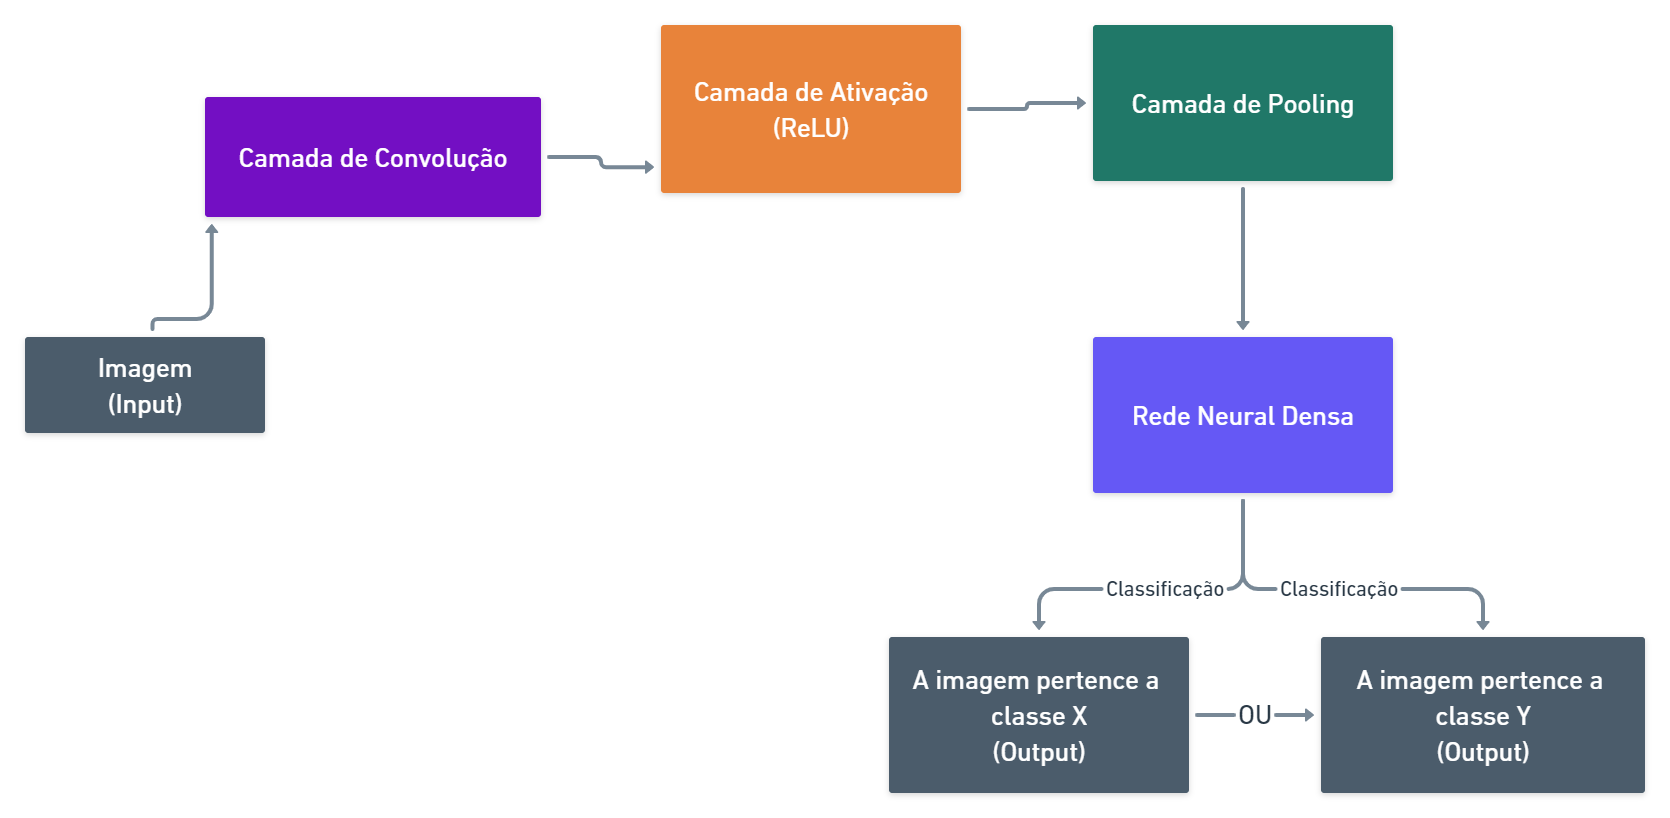
\includegraphics[width=1\textwidth]{CNN.png}
  \caption{O fluxo básico de uma CNN e suas diversas camadas.}
  \label{fig:exampleFig1}
\end{figure}


\subsection*{Convolução}

De modo geral a convolução é uma operação matemática realizada sobre duas funções resultando em uma terceira. Pode ser descrita em algoritmos de aprendizagem profunda pela função a seguir:

$$ S(i,j) = (I * K) (i,j) = \sum_m \sum_n I(m,n) K(i - m, j - n)  $$

\subsection*{Pooling}







% The first page must display the paper title, the name and address of the
% authors, the abstract in English and ``resumo'' in Portuguese (``resumos'' are
% required only for papers written in Portuguese). The title must be centered
% over the whole page, in 16 point boldface font and with 12 points of space
% before itself. Author names must be centered in 12 point font, bold, all of
% them disposed in the same line, separated by commas and with 12 points of
% space after the title. Addresses must be centered in 12 point font, also with
% 12 points of space after the authors' names. E-mail addresses should be
% written using font Courier New, 10 point nominal size, with 6 points of space
% before and 6 points of space after.

% The abstract and ``resumo'' (if is the case) must be in 12 point Times font,
% indented 0.8cm on both sides. The word \textbf{Abstract} and \textbf{Resumo},
% should be written in boldface and must precede the text.

% \section{CD-ROMs and Printed Proceedings}

% In some conferences, the papers are published on CD-ROM while only the
% abstract is published in the printed Proceedings. In this case, authors are
% invited to prepare two final versions of the paper. One, complete, to be
% published on the CD and the other, containing only the first page, with
% abstract and ``resumo'' (for papers in Portuguese).

% \section{Sections and Paragraphs}

% Section titles must be in boldface, 13pt, flush left. There should be an extra
% 12 pt of space before each title. Section numbering is optional. The first
% paragraph of each section should not be indented, while the first lines of
% subsequent paragraphs should be indented by 1.27 cm.

% \subsection{Subsections}

% The subsection titles must be in boldface, 12pt, flush left.

% \section{Figures and Captions}\label{sec:figs}


% Figure and table captions should be centered if less than one line
% (Figure~\ref{fig:exampleFig1}), otherwise justified and indented by 0.8cm on
% both margins, as shown in Figure~\ref{fig:exampleFig2}. The caption font must
% be Helvetica, 10 point, boldface, with 6 points of space before and after each
% caption.

% \begin{figure}[ht]
% \centering
% 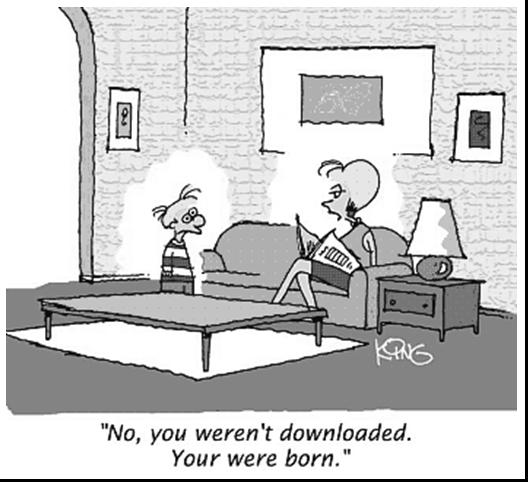
\includegraphics[width=.5\textwidth]{fig1.jpg}
% \caption{A typical figure}
% \label{fig:exampleFig1}
% \end{figure}

% \begin{figure}[ht]
% \centering
% 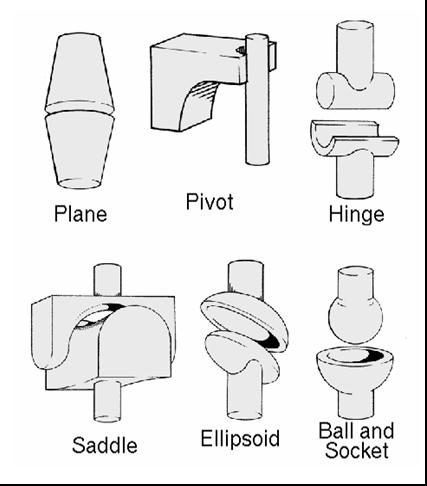
\includegraphics[width=.3\textwidth]{fig2.jpg}
% \caption{This figure is an example of a figure caption taking more than one
%   line and justified considering margins mentioned in Section~\ref{sec:figs}.}
% \label{fig:exampleFig2}
% \end{figure}

% In tables, try to avoid the use of colored or shaded backgrounds, and avoid
% thick, doubled, or unnecessary framing lines. When reporting empirical data,
% do not use more decimal digits than warranted by their precision and
% reproducibility. Table caption must be placed before the table (see Table 1)
% and the font used must also be Helvetica, 10 point, boldface, with 6 points of
% space before and after each caption.

% \begin{table}[ht]
% \centering
% \caption{Variables to be considered on the evaluation of interaction
%   techniques}
% \label{tab:exTable1}
% 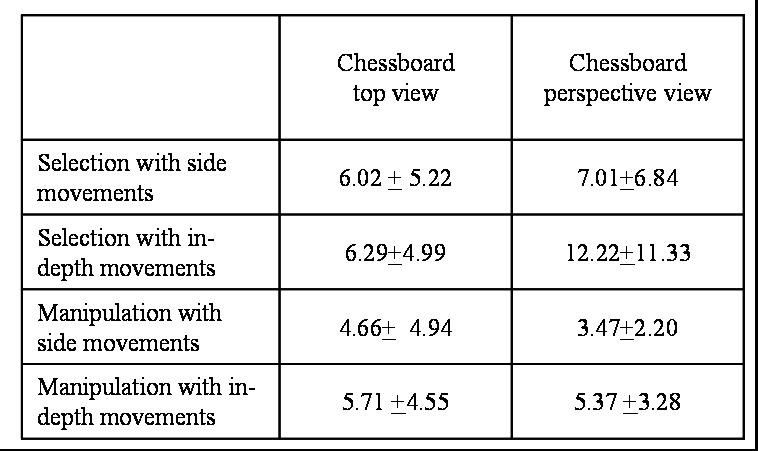
\includegraphics[width=.7\textwidth]{table.jpg}
% \end{table}

% \section{Images}

% All images and illustrations should be in black-and-white, or gray tones,
% excepting for the papers that will be electronically available (on CD-ROMs,
% internet, etc.). The image resolution on paper should be about 600 dpi for
% black-and-white images, and 150-300 dpi for grayscale images.  Do not include
% images with excessive resolution, as they may take hours to print, without any
% visible difference in the result. 

% \section{References}

% Bibliographic references must be unambiguous and uniform.  We recommend giving
% the author names references in brackets, e.g. \cite{knuth:84},
% \cite{boulic:91}, and \cite{smith:99}.

% The references must be listed using 12 point font size, with 6 points of space
% before each reference. The first line of each reference should not be
% indented, while the subsequent should be indented by 0.5 cm.

% \bibliographystyle{sbc}
% \bibliography{sbc-template}

\bibliographystyle{abnt}
\bibliography{sbc-template}

\end{document}